\section{Mjukvarulayout}
Efter diskussion med projektägare för att ta reda på kundens behov har en lista på funktioner och tjänster tagits fram. Varje funktion eller tjänst förklaras här nedan tillsammans med en motivation till varför vi anser att det bör vara en del av detta nätverk.

\subsection{IPSEC}
    Till att börja med måste det förklaras att det som tidigare nämnts som VPN-anslutning egentligen är ett privat nätverk som går mellan vissa siterna or core-siterna. Detta innebär att vissa siterna har koppling till varandra men inte ut på internet förutom via koppling till någon av core-siterna på detta privata nätverk.
    
\noindent Lösningen kommer oavsett vara att sätta upp en GRE-tunnel mellan siten och närmaste core-site, säkra denna med IPsec för att se till att alla paket är krypterade och kräva att all trafik går via core-siterna på väg ut mot internet. Detta ger att alla paket kan bli ordentligt undersökta eftersom den tuffare brandväggen kommer sitta centralt. Hastigheten på VPN-anslutningarna är rapporterat lägre vilket innebär att det på siter där det finns både internet och VPN-anslutning kommer internetanslutningen användas då den har högre hastighet och VPN-anslutningen kommer användas som backup.

\subsection{Port-säkerhet}
    Portar måste säkras både fysiskt och i mjukvara, och till det fysiska skyddet är tanken att använda sig av pluggade portar där man sätter in plastpluggar i portarna som gör att kablar inte går att sätta in där. Det finns även plastpluggar som man sätter på befintliga anslutna kablar, se Figur \ref{fig:rj45-caps}, som gör att kabeln inte går att dra ut utan att förstöra kabeln. Allt detta används för att förhindra datastöld och olaga intrång i switchar och routrar. När det kommer till mjukvarusäkerheten kommer de portar som inte används vara inaktiverade och på de portar som är i drift används 802.1x där varje användare som ska ansluta sig till det trådade nätverket behöver ett certifikat som godkänns delas ut av PKI-servern och autentiseras med RADIUS mot AD-servern.
    
    \begin{figure}[htb]
        \centering
        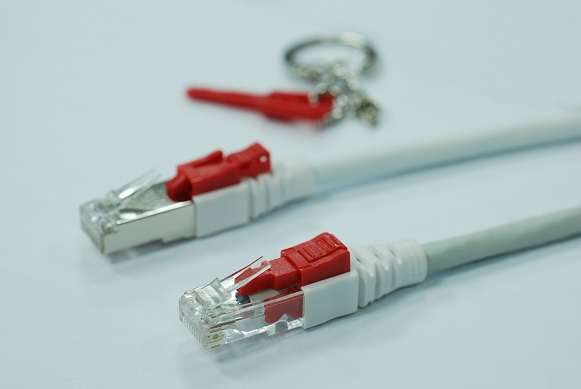
\includegraphics[width=0.5\textwidth]{pics/portsec.jpg}
        \caption[RJ45-lås]{Ett exempel på säkerhetslås för RJ45-kontakter.}
        \label{fig:rj45-caps}
    \end{figure}

\subsection{Admin-access \& Deployment}
    Admin-access kommer att lösas genom autentisering mot RADIUS där en användargrupp är konfigurerade som administratörer och med deras inloggningsuppgifter kan de logga in i alla enheter på alla siter. På enheterna kommer det även finnas ett lokalt konto för administratörer som backup ifall enheten inte kan nå RADIUS-servern. All kommunikation mellan administratörer och enheter sker över SSH version 2 och alla konfigurationstillfällen loggas centralt för att hålla reda på vem som gjort vad och när. \\
    
    \noindent Siterna finns i flera olika länder och utrustningen måste skeppas ner dit. När utrustningen transporteras ska det ej finnas någon konfiguration på dem eftersom paketet kan bli stulet. Skulle paketet bli stulet och det exempelvis är brandväggskonfiguration på enheten kan den som stjäl enheten se hur brandväggen är konfigurerad och då hitta eventuella säkerhetshål in i nätverket. Planen är istället att skicka enheterna till siterna helt tomma, och väl på plats koppla upp dem, ge dem en publik IP-adress för att de ska bli nåbara från en av core-siterna och därifrån skicka färdiga konfigurationer till enheten som läser in detta och sedan är klar för att kopplas ihop med det resterande nätverket.

\subsection{DNS}
    Alla core-siter kommer att ha en DNS-tjänst rullande på samma server som AD, vilket betyder att det kommer vara åtminstone en per core-site och dessa är redundanta mot varandra precis som AD är mellan core-siterna. Skulle mot förmodan alla DNS-servrar gå ner samtidigt kommer användarmaskinerna kopplas mot Fortiguards DNS (En säkerhetsfunktion som ingår i brandväggen) för att kunna ta sig ut på internet.

\subsection{Storm Control}
    Storm control har valts att läggas till som funktion i vår lösning för att det är en enkel och bra lösning som skyddar LAN från DOS-attacker eller dålig nätverkskonfiguration. Trafik som stormar, vare sig det är på grund av en angripare eller felaktig konfiguration, skapar onödig trafik på nätverket och degraderar nätverks prestanda. Konfiguration av Storm control på Fortinet-switchar är globalt på hela switchen och görs genom att specificera en maximal tröskel i paket per sekund (pps) \cite[48]{FN_FortiSwitch-Admin-Guide}. Om denna gräns överstigs blockar switchen några paket från att gå igenom tills pps har blivit mindre än den tillåtna tröskeln.

\subsection{NTP}
    Tidssynkronisering i nätverk är en väldigt viktig del när man ska administrera, säkra och lösa eventuella problem som kan uppstå i ett nätverk. Detta för att de flesta problem kan bara fastställas och lösas när man vet vad som hände och när det hände och utan den exakta tiden är det ofta omöjligt att bestämma var problemet ligger. NTP har valts som protokoll för tidssynkronisering för att det anses vara ett State of the Art tidssynkroniserings-protokoll och tidsförskjutningen är bara någon millisekund över internet och ännu lägre på ett lokalt LAN. NTP-servern är tänkt att bli placerad på core-siterna som sedan de mindre siterna synkroniserar sig emot. På grund av att NTP använder ett hierarkiskt system för synkronisering kan siter som tappar anslutning mot core fortfarande ha rätt tid då den närmsta enheten mot NTP-servern kommer bli ansvarig för synkronisering. Detta är viktigt eftersom tiden fortfarande då är rätt och synkad med andra enheterna i nätverket även när siten inte kan nå core.

\subsection{Loggning}
    Att sätta upp ett bra system för att övervaka och spara loggar i ett nätverk är kritiskt för både administration och säkerhet. I vår lösning har vi tänkt att spara loggar lokalt i 24 timmar för trafik som går igenom routrarna och sedan skicka de loggarna till en central loggserver på core. Om siterna inte kan nå core och ladda upp sin logg för de senaste 24 timmarna ska de sparas lokalt tills de kan kommunicera med core igen. Fortinet-enheter kör FortiOS och det erbjuder en robust loggningsmiljö där man kan övervaka, spara samt rapportera trafik och event som har med brandväggen att göra \cite{FN_FortiGate-Logging}. Man kan både välja att spara lokalt på enheten och skicka till en eller flera loggservrar.

\subsection{DHCP}
    En DHCP-server är tänkt att placeras ut lokalt på varje site för att dela ut IP-adresser för det spann som den siten är tilldelad. Genom att placera en DHCP-servern på varje site istället för på core kommer det leda till att de lokala enheterna på siterna fortfarande kan få en IP-adress tilldelad även om den siten inte kan nå core. FortiGate 60E på varje site kommer att användas som den lokala DHCP servern för att den är enkel att konfigurera och behöver man inte ha någon extra server bara för DHCP.

\newpage
\subsection{Firewall}
    FortiGate har en inbyggd brandvägg med IPS och threat protection \cite{FN_FortiGate-60E}. Med hjälp av FortiGuard kan varje FortiGate snabbt uppdatera dess signaturlistor för kända virus, trojaner och maskar att blockera. FortiGuard har också ett inbyggt App Control-system för eventuella begränsningar av förbjudna program eller tjänster. FortiGate 60E-PoE-modellen kan med alla tjänster aktiverade skyffla 200 Mbps av data, väl tillräckligt för det satta minimikravet.

\subsection{FortiClient}
    FortiClient är Fortinets egna program för end-point-skydd, dvs ett antivirusprogram för klienter \cite{FN_FortiClient}. FortiClient använder FortiGuard för att enkelt kunna uppdatera dess signaturlista. Dock är det upp till användarna att säkra sin utrustning för att vi inte har någon kontroll över deras enheter så vi kan endast rekommendera ett antivirus skydd.

\subsection{RADIUS}
    FortiGates kan enkelt konfigureras så att klienter ska autentisera med vald metod (MS-CHAP, CHAP, PAP) till en RADIUS server. Helst bör ett autentiserat certifikat användas för att säkerställa att RADIUS servern är genuin.

\subsection{NAT}
    NAT används inom hela nätverket då kanske endast ett eller ett fåtal publika IP-adresser finns tillgängliga och alla enheter samt klienter använder privata adresser. Dock behöver siternas routrar inte behandla NAT då enligt vår föreslagna design konverteras all NAT-trafik hos core-siterna innan data skickas ut på publikt internet.
